\chapter{Cahier de Charges et Analyse}

\section*{Introduction}%
\addcontentsline{toc}{section}{\numberline{}Introduction}%
Comme son nom ce chapitre a pour but de ressortir les différents éléments présents dans le cahier de charges d’un projet. Nous allons commencer par étudier la problématique dont fait face l’entreprise et de là nous allons faire une étude de l’existant. Le résultat de ceci nous guidera dans le choix d’une solution que nous allons présenter, puis nous allons analyser la solution pour en ressortir les fonctionnalités. De là nous seront en mesure de faire une planification pour notre projet ainsi qu’une estimation des couts.
\section{Problématique}
\subsection{Présentation du cas d’études : AMD Sarl}
AMD est l'agent / distributeur exclusif au Cameroun de plusieurs categories de materiaux de maintenance industrielle. De ce fait la gestion commerciale est un element cle dans la survie economique de l'entreprise. AMD Sarl est une PME et comme la plupart des entreprises, pour leur aider dans la gestion de leurs activités au quotidien y compris la gestion commerciale, ils utilisent un outil de gestion commerciale en ligne, notamment l’ERP\footnote{Enterprise Resource Planning (Progiciel de Gestion Intégré en français)} Sage 100.
Cependant l'entreprise a souvent besoin d'optimiser le processus de fixation des prix de leurs produits ou encore savoir a quel moment avoir un certain produit en stock, ce qui pourrait nettement améliorer les ventes de l'entreprise. Ceci est rarement optimal. De ce fait ca devient plus difficile pour l'entreprise de fidéliser les clients ou encore acquérir des nouveaux clients. 
\subsection{Démarche d’analyse du problème}
Pour mieux analyser notre problème, on a résolu à utiliser la méthode des 5M. Aussi appelé diagramme de causes/effets" ou "en arêtes de poisson", l'outil créé par Mr Ishikawa fait partie de ceux à posséder dans sa trousse à outils spéciale "résolution des problèmes". Rappelant le squelette d'un poisson, cet outil visuel a pour finalité de lister les causes qui ont une influence sur un effet (une situation), de les classer, de les hiérarchiser. Très utilisé par les qualiticiens, le diagramme d'Ishikawa est en fait applicable à l'ensemble des métiers de l'entreprise.
\paragraph{}
Les étapes principales dans l’utilisation de cette méthode sont les suivants :
\begin{itemize}
    \item \textbf{Qualifiez l'effet :} Il s'agit couramment du problème que vous cherchez à résoudre. Dans notre contexte on peut identifier les effets suivants :
    \begin{itemize}
        \item La diffculté à fixer un prix pouvant generer un gain maximal à un moment précis
        \item Savoir a quel moment avoir un produit en particulier en stock et la quantité pour éviter des clients insatisfaits.
    \end{itemize}
    \item \textbf{Dressez un inventaire des causes possibles }: Il s’agit de lister les causes qui ont une influence sur le problème. Dans notre contexte on peut constater que l'entreprise possède des données généres par ses systèmes de gestion qui ne sont pas exploitées. De ce fait il ya un maque d'outils pouvant aider à faire des décisions.
    \item \textbf{Classez les causes par familles :} Ici intervient les 5M qui sont fréquemment utilisés pour cette tâche : Main d’œuvre, matière, matériels, méthodes, milieu. Dans notre cas on a une seule catégorie qui est la méthode d'utilisation de nos données.
    \item \textbf{Evaluez les branches/racines qui ont le plus d'impact.}
\end{itemize}

Le diagramme Ishikawa dans la figure \ref{fig:ishikawa} nous montre l'origine des problématiques dont fait face l'entreprise.
\begin{figure}[H]
    \centering
    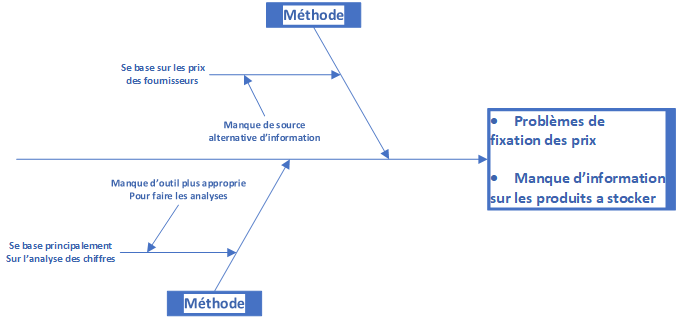
\includegraphics[width=\textwidth]{ishikawa}
    \caption{Diagramme Ishikawa analysant nos problématiques}
    \label{fig:ishikawa}
\end{figure}


\subsection{Identification de la problématique}
L’entreprise possède une quantité énorme d’informations non exploités, qui peuvent non seulement optimiser la prise de décisions par les décideurs mais aussi faciliter le travail des employés, augmentant ainsi la productivité de celles-ci, si exploitée de la bonne façon. 

De ce fait on peut identifier les problématiques suivantes, aussi représentés dans la figure 
\begin{itemize}
    \item La difficulté à fixer le prix d'un produit pour avoir un revenue maximal sur celui ci dans période bien précise.
    \item La difficulté dans l'identification des produits à mettre en stock avec les quantités à une certaine période pour éviter d'avoir des clients qui commandent des produits qu'on ne peut pas fournir.
\end{itemize}



\section{Etude de l’existant}
Nous ne saurions débuter ce travail sans avoir une idée claire et précise sur l’existant quel qu’il soit. La première tâche a été de rencontrer les différentes personnes qui sont ou peuvent être impliquées dans les prises de décision et la gestion commerciale en général dans l’entreprise. 
\paragraph{}
Nous avons principalement travaillé avec le chef du département de l’approvisionnement, de la recherche et de l’innovation, M. Arnold KOGAING. Après quoi, nous avons réellement débuté le travail en menant différentes recherches. Cette méthodologie de travail nous a permis d’avoir une connaissance large de l’existant.

\subsection{La gestion commerciale à AMD}
AMD Sarl est une PME et comme la plupart des entreprises, pour leur aider dans la gestion de leurs activités au quotidien y compris la gestion commerciale, utilisent un outil de gestion commerciale en ligne, notamment l’ERP Sage 100.
\paragraph{}
Sage 100 est un logiciel qui propose d’accompagner les petites et moyennes entreprises dans la gestion de leurs ressources. De la gestion commerciale en passant par la comptabilité et les fonctionnalités de pilotage, Sage 100 s’impose comme un outil indispensable aux PME. Pour autant, la gestion des clients tout comme celle des achats et des fournisseurs ne sont pas en reste puisque Sage 100 propose une gestion puissante du cycle de vente du début de la chaîne jusqu’à sa fin.
\paragraph{}
Sage 100 est assez récent dans l’entreprise avec d’autres outils tels Gescom v14 et MS Excel utilisés pour gérer les processus de gestion commerciale. 

\subsubsection{Outils de gestion commerciale}
Le tableau \ref{tab:outilsdegescom} decrit un peu l'historique des outils des gestion commerciale utilisés par AMD.

\begin{table}[H]
    \centering
    \caption{Tableau des outils de gestion commerciale utilisés au fil du temps.}
    \begin{tabular}[t]{|p{3cm}|p{7cm}|p{5cm}|} 
        \hline
        \textbf{Outil} & \textbf{Description} & \textbf{Période} \\
        \hline\hline
        Sage 100 & ERP offrant de nombreuses fonctionnalitées & Moins de 10 mois d'utilisation \\
        \hline
        Gescom v14 & ERP, offrant moins de fonctionnalites que Sage 100 et les données sont moins descriptifs. Données pas aussi  fiables que celles de Sage 100  & Utilisation sur 3 années avant Sage 100 \\ 
        \hline
        Microsoft Excel & Tableur, permettant de concevoir de modèle de gestion assez complexes. Données encore moins fiables que celles de Gescom v14 & Utilisation sur 10 ans avant Gescom v14 \\ 
        \hline
        Traces papiers & Utilisation de papiers pour garder toute traces des transactions effectués par l’entreprise. & Dès la création de l’entreprise jusqu’à l’introduction de MS Excel. \\ 
        \hline\hline
    \end{tabular}
    \label{tab:outilsdegescom}
\end{table}%

\subsubsection{Prises de décisions en gestion commerciale}
Concernant de départements en entier, les décisions finales sont prises par le directeur général de l’entreprise après une ou plusieurs réunions avec les responsables dans le département en question et d’autres cadres. Ces réunions incluent souvent des brainstormings ou encore des analyses des chiffres. Il peut aussi arriver que le directeur se fie à son intuition pour prendre une décision. La figure \ref{fig:niveaudeladecision}, extraite d'un document en ligne\footnote{http://mmanagement.e-monsite.com/medias/files/les-decisions-et-parties-prenantes.pdf} intitulé \textit{"Décisions et le processus de décision"} montre les niveaux de décisions en entreprise.

\begin{figure}[H]
    \centering
    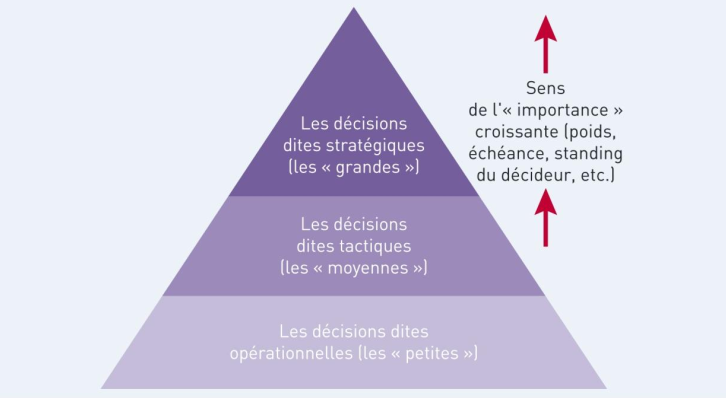
\includegraphics[width=\textwidth]{niveaudeladecision}
    \caption{Les niveaux de la décision}
    \label{fig:niveaudeladecision}
\end{figure}


Pour les décisions moins importantes, les chefs des différents départements ou services peuvent s’en charger suivant le même procédé que celui mentionné plus haut. En gros on recueille les points suivants dans la procédure de prise de décision.
\begin{itemize}
    \item Identifier la problématique à résoudre
    \item Identifier les différentes options possibles (brainstormings)
    \item Analyser les conséquences pour chaque option (analyses des chiffres)
    \item Définir l'option retenue (le directeur) et la mettre en oeuvre (les acteurs concernés)
\end{itemize}

\subsection{Critique de l’existant}
La critique de l'existant, appelée aussi bilan de l'existant, va nous aider à l'évaluation du système existant par rapport à la prise de décisions de gestion commerciale puisque c'est là que se pose nos problématiques. Ce diagnostic est établit dans le but de rechercher des solutions futures à des problèmes posés.
\paragraph{}
Le but de la critique de l'existant est d'établir un diagnostic précis sur les procédures utilisées, relever les anomalies, les qualités et les défauts du système existant.
\paragraph{}
Par ailleurs, deux aspects sont toujours dégagés lors de cette critique dont l'un est positif et l'autre négatif.Ces deux aspects méritent d'être soulevés étant donné que le besoin de la perfection sera toujours souhaité par les utilisateurs en vue de bon fonctionnement.

\subsubsection{Aspect(s) positifs}
Sous forme de liste on peut recenser les points positifs suivants dans le processus de prise de décisions.
\begin{itemize}
    \item Les opinions et analyses sont collectives
    \item Les chiffres (données) sont prises en considération dans le processus
    \item L'aspect \textit{"intuition"} est aussi considéré, ce qui garde notre nature humaine dans le processus.
\end{itemize}

\subsubsection{Aspect(s) négatifs}
Dans le processus de prise de décisions, l'analyse des chiffres intervient mais comme nous le savons tous, l'erreur est humaine. En ce faisant on peut rencontrer l'un des problèmes suivants, ce qui risque de mener à une mauvaise décision :

\begin{itemize}
    \item Mauvaise compréhension des chiffres
    \item Mauvaise correlation entre les différents sources ou rapports
    \item Ne pas analyser au delà des chiffres
    \item Focus sur la mauvaise métrique
\end{itemize}


\subsection{Les solutions concurrentes}
Nous avons vu plus haut les étapes du processus de prise de décisions. Il peut être reformulé de la façon suivante :
\begin{itemize}
    \item La phase de formulation ;
    \item La phase d’instruction ;
    \item La phase de choix ;
    \item La phase d’exécution.
\end{itemize}
\subsubsection{Techniques de prise de décisions}
Dans le processus mentionné plus haut c’est la troisième phase qui nous intéresse ici. On recense les techniques suivantes pour passer cette phase :
\begin{itemize}
    \item Se fier à l’intuition d’une ou plusieurs personnes
    \item Analyser les chiffres
    \item Utiliser un outil d’aide à la décision (Business Intelligence)
\end{itemize}

Nous avons vu plus haut quelques problèmes sur lesquels nous pouvons tomber en simplement analysant les chiffres sans outil d’aide. Aussi, l’intuition humaine peut s’avérer important dans certaines situations mais il est loin d’être suffisant pour prendre des décisions importantes. Nous pouvons ainsi conclure qu’un outil d’aide à la décision s’impose si nous voulons être optimal dans nos prises de décisions.

\subsubsection{Typologies des solutions de Business Intelligence}
\begin{itemize}
    \item \textbf{BI intégrée :} Il s’agit de solutions pouvant être intégrées à d’autres applications. Elle offrent des fonctionnalités analytiques et génèrent rapports et tableaux de bords ad hoc. Leur grande force réside dans leur capacité à s’intégrer à l’existant, y compris aux solutions de gestion d’éditeurs différents.
    \item \textbf{BI en libre service :} Il s’agit de solutions orientées utilisateur final : il n’a pas à se soucier du traitement en amont des données. Par le biais d’une interface conviviale, il peut librement explorer les données disponibles via des tableaux de bords personnalisables. On qualifie parfois ces solutions d’auto-suffisantes car elles accèdent à différentes sources de données pour en extraire des informations pertinentes sans le concours d’un service informatique dédié.
    \item \textbf{La DataViz :} Il s’agit de la data visualisation (visualisation de données) une fonction essentielle dans le traitement graphique des données traitées par la BI. Il s’agit de rendre intelligibles les informations traitées sous formes de graphes, tableaux et autres histogrammes. L’utilisateur final peut à loisir opter pour la visualisation qui correspond au traitement attendu des données. Contrairement à d’autres solutions, les applications de DataViz ne se connectent pas à des entrepôts de données non-structurées mais utilisent des bases de données déjà établies et/ou les données issues d’applications métiers. Il s’agit de fournir des indicateurs précis en temps réel afin de saisir un instantané opérationnel. La plupart du temps les tableaux de bord offrent une interface qui permet de les modifier par simple glisser-déposer.
    \item \textbf{Plate-forme de Business Intelligence : } Il s’agit d’outils complets de traitement des données structurées et non-structurées. Ils exploitent ces dernières afin d’en tirer une analyse pertinente, traduite elle aussi sous forme graphique. Ce type de solutions nécessite souvent un travail de développement et des spécialistes au sein d’un service informatique qui géreront le traitement des données en amont de l’utilisateur métier. Ce dernier peut alors se consacrer pleinement à l’analyse métier.
\end{itemize}
Nous avons plusieurs sources de données de différents types, nous voulons pouvoir faires des analyses et enfin visualiser ces données. Après cette étude nous sommes ressortis avec le tableau \ref{tab:comparatiftypebi} comparant les différents types de BI. Ceci nous guidera dans notre choix du type de solution à adopter.

\begin{table}[H]
    \centering
    \caption{Tableau comparatif des types de Business Intelligence.}
    \begin{tabular}[t]{|p{6cm}|p{3cm}|p{3cm}|p{3cm}|} 
        \hline
        \textbf{Typologie} & \textbf{Agrégation} & \textbf{Analyse} & \textbf{Visualisation} \\
        \hline\hline
        BI intégrée & Non & Non & \textbf{Oui} \\
        \hline
        BI en libre service & Non & Non & \textbf{Oui} \\
        \hline
        La DataViz & Non & \textbf{Oui} & \textbf{Oui} \\
        \hline
        Plate-forme de Business Intelligence & \textbf{Oui} & \textbf{Oui} & \textbf{Oui} \\
        \hline\hline
    \end{tabular}
    \label{tab:comparatiftypebi}
\end{table}%



\section{Solution retenue}
Nous constatons donc que la typologie qui répond pleinement a nos attentes est la plate-forme de Business Intelligence. Nous allons donc opter pour cette option et commencer la construction de notre plate-forme.

\subsection{Description de la solution}
Le terme Business Intelligence (BI), ou informatique décisionnelle, désigne les applications, les infrastructures, les outils et les pratiques offrant l’accès à l’information, et permettant d’analyser l’information pour améliorer et optimiser les décisions et les performances d’une entreprise. Le schéma dans la figure \ref{fig:aidealadecision} extrait d'une présentation de Ronan Tournier sur ResearchGate\footnote{https://www.researchgate.net/figure/Architecture-dun-systeme-decisionnel-fig2-30514732} montre la place que le système vient occuper dans l'entreprise.

\begin{figure}[H]
    \centering
    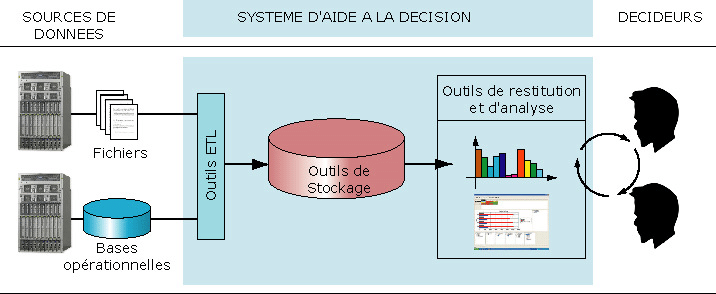
\includegraphics[width=\textwidth]{aidealadecision}
    \caption{Le système d'aide à la décision.}
    \label{fig:aidealadecision}
\end{figure}

Ainsi, la BI regroupe une large variété d’outils, d’applications et de méthodologies permettant de collecter des données en provenance de systèmes internes et de sources externes, de les préparer pour l’analyse, de les développer et de lancer des requêtes au sein de ces ensembles de données. Ces outils permettent ensuite de créer des rapports, des tableaux de bord et des visualisations de données pour rendre les résultats des analyses disponibles pour les preneurs de décisions.
\paragraph{}

De ce fait notre solution sera constitué de trois (03) grandes parties, chaqu’une pouvant être implémentée indépendamment avec des outils qui lui sont propres.  
\begin{itemize}
    \item \textbf{Agrégation des données :} Cette partie concerne la construction de l’entrepôt de donnes ou datawarehouse, à partir des multiples sources de données. On utilisera les notions d’ETL abordées plus haut dans la revue de littérature. La finalité de cette partie est un dépôt central de données structuré prêt à être utilisé à des fins d’analyse.
    \item \textbf{Analyse des données :}  Ici nous allons nous concentre sur l’aspect d’analyse des données pour en ressortir l’information souhaitée. Nous allons nous baser sur des problématiques précises pour faire nos analyses et ressortir des indicateurs. On utilisera les concepts de Datamart et cubes OLAP pour faire nos analyses. Dépendant des problématiques posées en entrée, nous en ressortons d’ici avec des indicateurs prêts à être utilise dans un outil de visualisation de données.
    \item \textbf{Reporting (Visualisation des données) :} C’est la partie la plus intéressante pour l’utilisateur final. Se basant sur des indicateurs, on conçoit des rapports et tableaux de bords personnalisables pour donner une meilleure vue a l’utilisateur sur les données. C’est ce qui permet à l’utilisateur final de mieux comprendre les données et prendre des meilleures décisions.
\end{itemize}


\subsection{Objectifs du projet final}
Après avoir posé nos problèmes et étudié comment nous allons procéder à leurs résolutions, nous pouvons à présent parler des objectifs de notre solution.

\subsubsection{Objectif général}
L’objectif général c’est de mettre sur pied une plateforme de Business Intelligence, de l’intégration des données jusqu’à la visualisation en passant par l’analyse. 

\subsubsection{Objectifs spécifiques}
La solution devra nous permettre de :
\begin{itemize}
    \item Intégrer des données provenant de diverses sources notamment, l’ERP Sage 100, Gescom v14 et des fichiers Excel.
    \item Faire des analyses multidimensionnelles sur nos données.
    \item Visualiser nos données en masse et en ad hoc.
\end{itemize}










\section{Analyse Fonctionnelle (A.F.)}
L’A.F. s’adresse aux concepteurs de produits. Il peut s’agir d’un objet matériel ou immatériel (produit industriel, objet technique, service à la personne, services financier, programme informatique dans notre cas...). Le but de l’AF est d’optimiser la conception ou la reconception de produits en s’appuyant sur les fonctions que doit réaliser le produit. Une fois les fonctions du produit identifiées et caractérisées, l’équipe de conception peut mesurer son état d’avancement et de réussite par rapport à des critères objectifs.

\subsection{La démarche d’analyse fonctionnelle (A.F.)}
L’AF n’a de sens que si elle est menée au début d’un projet. Elle permet d’éviter certains pièges classiques de la conception (aveuglement, manque d’objectivité, mauvaise gestion des priorités). Dans les faits, les premières étapes de l’AF sont générales et concernent tous les acteurs d’un même projet. C’est seulement dans un deuxième temps qu'elle devient technique, et oriente les concepteurs vers des solutions techniques. Rendant ainsi possible un dialogue entre tous les intervenants d’un projet (quels que soient leurs domaines de compétence). C’est un gage d’objectivité et de créativité dans la conduite du projet.

\subsubsection{La méthode APTE : \textbf{AP}plication aux \textbf{T}echniques d’\textbf{E}ntreprise}
La méthode APTE est une méthode « universelle » d’aide à la gestion de projets, enseignée et/ou dispensée de façon très officielle par l’APTE, cabinet conseil en management, spécialisé en Analyse de la Valeur. D'apres le site officiel de la methode\footnote{http://www.methode‐apte.com/}, elle est une interprétation française de méthodes américaines d’analyse de la valeur.

\subsubsection{Les étapes de l’A.F.}
Lors d’une démarche d’analyse fonctionnelle, les concepteurs (au sens large) du produit doivent suivre les étapes suivantes, présentées dans l’ordre chronologique.
\begin{table}[H]
    \centering
    \caption{Etapes à suivre dans l'Analyse Fonctionnelle.}
    \begin{tabular}[t]{|p{6cm}|p{9cm}|} 
        \hline
        \textbf{Outil} & \textbf{Résultat attendu}\\
        \hline\hline
        Analyse du Besoin (A.B.) & Cahier des charges du besoin (note de
        cadrage). \\
        \hline
        Analyse Fonctionnelle du Besoin (A.F.B.) & Cahier des charges fonctionnel \\
        \hline
        Analyse Fonctionnelle Technique (A.F.T.) & Cahier des charges technique (spécification
        technique).\\
        \hline\hline
    \end{tabular}
    \label{tab:etapesaf}
\end{table}%

Le tableau \ref{tab:etapesaf} ressort les étapes nécessaire à l'A.F. ainsi que le résultat dont on doit espérer à la fin de chaque étape.
\begin{itemize}
    \item L’Analyse du Besoin permet \textbf{d’exprimer le besoin}.
    \item L’Analyse Fonctionnelle du Besoin permet d’identifier les relations du produit avec son contexte d’utilisation, afin de dégager des \textbf{Fonctions de Service}, aptes à satisfaire le besoin.
    \item L’Analyse Fonctionnelle Technique permet de déterminer les \textbf{Fonctions Techniques} nécessaires aux fonctions de service. Ces fonctions techniques guident les concepteurs dans la recherche des \textbf{solutions technologiques}.
\end{itemize}
\paragraph{}
L’Analyse Fonctionnelle du Besoin porte sur les \textbf{fonctions} du produit à concevoir. Elle ne préjuge pas ni des fonctions techniques induites ni des solutions constructives capables qui seront recherchées au stade de l’Analyse Fonctionnelle Technique.
\paragraph{}
La démarche d’Analyse Fonctionnelle (AB, AFB et AFT) est collective, et doit réunir des personnes représentant tous les services et tous les métiers concernés. Cela permet à la fois plus de créativité, et d’exhaustivité dans la démarche. La réflexion doit rester la plus ouverte possible, tout au long de la démarche d’analyse.

\subsection{L'Analyse du Besoin (A.B.)}

\subsubsection{Définition}
« Un besoin est un désir (ou une nécessité) éprouvé par l’utilisateur d’un système », selon AFNOR\footnote{AFNOR - Association Française de Normalisation}
\paragraph{}
On recense deux formes principales de besoin : 
\begin{itemize}
    \item Explicite (Exprimé)
    \item Implicite (Non Exprimé)
\end{itemize}

\subsubsection{Verbalisation du besoin}
La méthode de l’Analyse du Besoin s’appuie sur deux hypothèses :
\begin{itemize}
    \item La satisfaction du besoin est réalisée par l’utilisation du produit à concevoir.
    \item Le besoin est satisfait par le changement d’état d’une matière d’œuvre.
\end{itemize}

Pour verbaliser le besoin, il faut se poser trois questions et y répondre. Le tableau ... montre, dans notre projet les questions et les réponses qui nous mèneront à la formulation de notre besoin.

\begin{table}[H]
    \centering
    \caption{Questions pour formuler le besoin.}
    \begin{tabular}[t]{|p{7cm}|p{8cm}|} 
        \hline
        \textbf{Question} & \textbf{Réponse}\\
        \hline\hline
        « \textbf{A qui} le produit rend‐il service ? » & Aux décideurs \\
        \hline
        « \textbf{Sur quoi} le produit agit‐il ? » & Les données de gestion commerciale \\
        \hline
        « \textbf{Dans quel but} ? » & Améliorer la prise de décisions\\
        \hline\hline
    \end{tabular}
    \label{tab:etapesaf}
\end{table}%

Traditionnellement dans la méthode APTE le besoin est représenté grâce à un outil graphique : le schéma du besoin (la « Bête à cornes ») illustré dans la figure \ref{fig:bac}.

\begin{figure}[H]
    \centering
    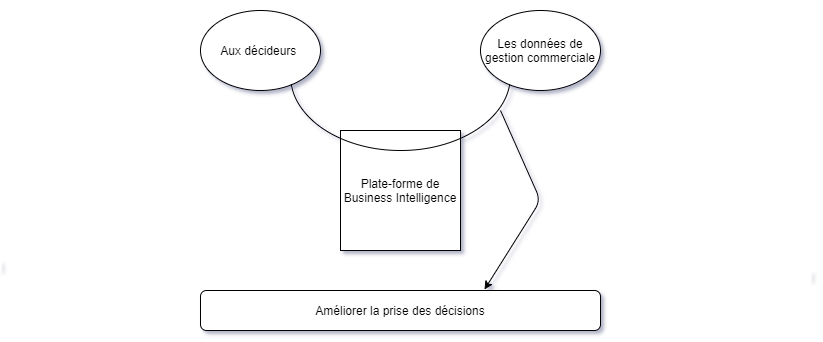
\includegraphics[width=\textwidth]{bac}
    \caption{Diagramme bête à cornes}
    \label{fig:bac}
\end{figure}

Les réponses à ces trois questions aboutissent à un énoncé du besoin, qui peut être formulé comme suit :

\textbf{« La plate-forme de Business Intelligence rend service aux décideurs de AMD Sarl en agissant sur les données de gestion commerciale pour améliorer la prise des décisions »}.



\subsection{L'Analyse Fonctionnelle du Besoin (A.F.B.)}
L'A.F.B est faite selon les deux hypothèses suivantes :
\begin{itemize}
    \item Le besoin est satisfait par l’utilisation d’un produit.
    \item Le produit est un générateur de \textbf{services} (ou « prestations client »)
\end{itemize}

\subsubsection{Les concepts de l’A.F.B}
L’Analyse Fonctionnelle du Besoin est appelée ainsi car elle va permettre de traduire le besoin en des fonctions à réaliser : les \textbf{Fonctions de Service}. L'A.F.B. est aussi appelée Analyse Fonctionnelle Externe.
\paragraph{Notion de Fonctions de Service (F.S.)}
Définition d’une fonction suivant la norme AFNOR X50‐151 :
\textbf{« Action d'un produit ou de l'un de ses constituants exprimée exclusivement en termes de finalité ».}
\subparagraph{}
On peut l'interpreter comme une action du produit avec son milieu extérieur, qui contribue à la satisfaction du besoin (identifié et caractérisé lors de l’A.B.). On ne peut identifier et caractériser les fonctions de service que si l’on a au préalable \textbf{identifié et caractérisé le milieu extérieur} du produit. Le milieu extérieur du produit à concevoir dépend de l’instant auquel on le considère. Le cycle de vie du produit étant constitué de multiples étapes, on doit identifier le \textbf{milieu extérieur correspondant à chaque phase de vie du produit.}

\paragraph{Les étapes de l’A.F.B.}
L’Analyse Fonctionnelle du Besoin est une démarche relativement longue, qui conditionne
grandement la réussite du projet et demande donc beaucoup de rigueur et de soin.
\begin{itemize}
    \item Identification des \textbf{phases de vie} du produit
    \item Pour chaque phase de vie (à minima les principales) :
    \begin{itemize}
        \item Identification et caractérisation des \textbf{Eléments du Milieu Extérieur (E.M.E.)}
        \item Identification des Fonctions de Service (F.S.)
        \item Caractérisation des F.S.
    \end{itemize}
    \item Rédaction du \textbf{cahier des charges fonctionnel}
\end{itemize}

\subsubsection{Phases de vie du produit}
Suivant les objectifs de la conception et le niveau de précision recherché, on peut identifier
de très nombreuses phases de vie pour un produit.

On peut avoir conception, fabrication, tests d’intégration, conditionnement, transport, commercialisation, montage, installation / mise en œuvre, validation, utilisation normale (principale), utilisation normale (secondaire), utilisation anormale (mode dégradé), maintenance, non utilisation, stockage, reconditionnement, mise à jour, recyclage / destruction. Cete liste est non exhaustive.

Dépendant des objectifs du  produit on peut choisir les phases de vie de notre produit.

Notre produit est une solution informatique. On peut donc se baser sur le cycle de vie d'un logiciel informatique déjà conçu pour choisir les phases de vie de notre produit.

On peut donc choisir les suivants : 
\begin{itemize}
    %\item conception
    \item utilisation
    \item mise à jour
\end{itemize}

\subsubsection{Eléments du Milieu Extérieur (E.M.E.)}
Pour identifier les fonctions du produit, il faut être capable de décrire son environnement (appelé « Milieu Extérieur »). Toutes les entités qui sont identifiées comme extérieures au produit
sont appelées \textbf{Eléments du Milieu Extérieur : E.M.E.}. Les E.M.E. doivent être identifiés pour chaque phase de vie étudiée!

Pour ce faire il faut identifier les éléments intervenant dans chaque phase de vie et en déterminer les E.M.E. Un E.M.E. doit pouvoir être défini de façon objective pour tous les protagonistes de l’étude. Si on ne peut pas définir entièrement un élément par des critères objectifs, alors cet élément n’est pas un élément du milieu extérieur. Le choix d’un E.M.E. conditionnera l’énoncé des Fonctions de Service.

% \paragraph{Phase de conception}
% Ici on peut identifier comme éléments dans l'environnement du produit les suivants:
% \begin{itemize}
%     \item Outils de conception
%     \item Modèle de données
%     \item Concepteur
%     \item Normes de sécurité 
%     \item Règles de qualité
% \end{itemize}
% On aura donc un diagramme comme dans la figure \ref{fig:emeconception}


% \begin{figure}[H]
%     \centering
%     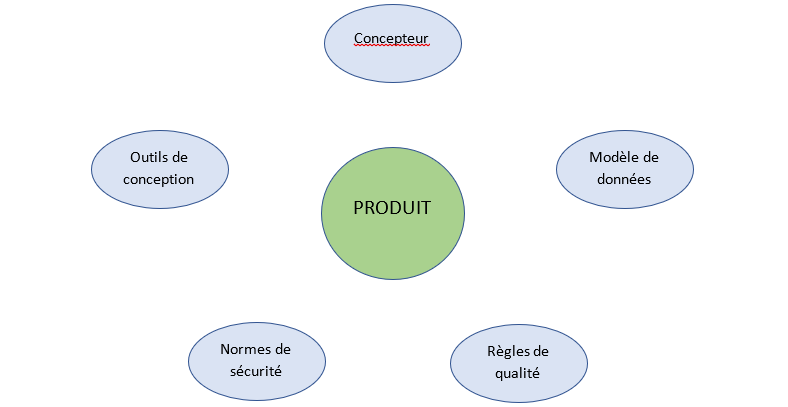
\includegraphics[width=\textwidth]{emeconception}
%     \caption{Identification des E.M.E. dans la phase Conception}
%     \label{fig:emeconception}
% \end{figure}

\paragraph{Phase d'utilisation}
Ici on peut identifier comme éléments dans l'environnement du produit les suivants:
\begin{itemize}
    \item Client 
    \item Données
    \item Décisions
    \item Normes de sécurité 
    \item Normes d'ergonomie
    \item Règles de qualité
\end{itemize}
On aura donc un diagramme comme dans la figure \ref{fig:emeutilisation} représentant les E.M.E.

\begin{figure}[H]
    \centering
    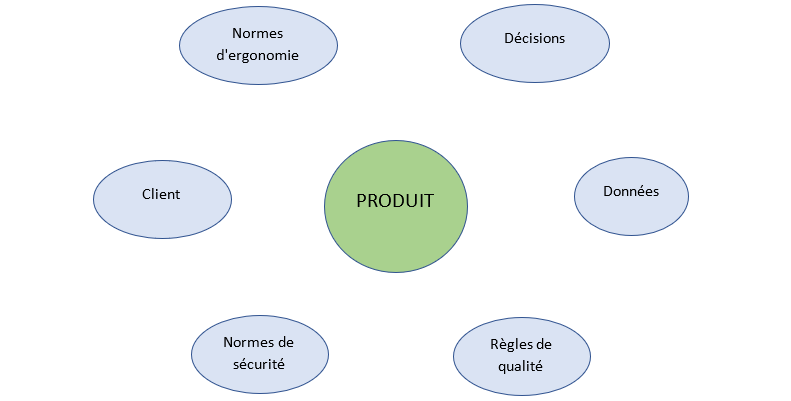
\includegraphics[width=\textwidth]{emeutilisation}
    \caption{Identification des E.M.E. dans la phase Développement}
    \label{fig:emeutilisation}
\end{figure}



\paragraph{Phase de mise à jour}
Ici on peut identifier comme éléments dans l'environnement du produit les suivants:
\begin{itemize}
    \item Client (Décideurs) 
    \item Données 
    \item Décisions 
    \item Concepteur
    \item Normes de sécurité 
    \item Normes d'ergonomie
    \item Règles de qualité
\end{itemize}
Ici on peut constater que le client et les données en sont pas intrinsèquement liées à la phase de mise à jour. On a donc Client et Données comme E.M.E. ici. On aura donc un diagramme comme dans la figure \ref{fig:ememiseajour}.


\begin{figure}[H]
    \centering
    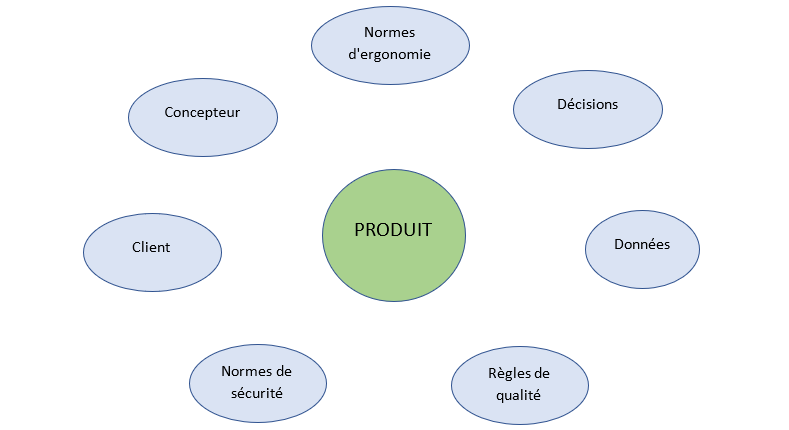
\includegraphics[width=\textwidth]{ememiseajour}
    \caption{Identification des E.M.E. dans la phase Mise A Jour}
    \label{fig:ememiseajour}
\end{figure}



\subsubsection{Fonctions de Service (F.S.)}
On identifie les Fonctions de Service grâce à un outil graphique : le graphe des interacteurs,
ou graphe fonctionnel (le « Diagramme Pieuvre » de la méthode APTE) :
\begin{itemize}
    \item Les relations du produit avec son milieu extérieur (pour une phase de vie donnée) sont représentées par des traits.
    \item Chaque trait correspond à une Fonction de Service (F.S.)
    \item Chaque trait doit relier le produit à un EME ou bien relier plusieurs EME en passant par le produit.
\end{itemize}

\paragraph{Classification des Fonctions de Service}
\begin{itemize}
    \item \textbf{Fonctions Principales (F.P) : \textit{« Fonction de service qui met en relation deux EME (ou plus), via le produit »}.} Les fonctions principales traduisent obligatoirement des actions réalisées par le produit. Il peut être nécessaire de mettre en relation plus de deux EME par une seule fonction principale, mais c’est un cas à éviter dans la mesure du possible.
    \item \textbf{Fonctions Contraintes (F.C) : \textit{« Fonction de service qui met en relation le produit avec un seul EME »}.} Chaque EME doit être relié au produit par au moins une fonction contrainte. Les fonctions contraintes traduisent la plupart du temps une adaptation du produit à son milieu
    extérieur.
\end{itemize}

\paragraph{L’expression des fonctions est normalisée par l’AFNOR :} Une fonction se compose d'un \textbf{verbe} ou d'un \textbf{groupe verbal caractérisant l'action}, et de compléments représentant les \textbf{éléments du milieu extérieur} concernés par la fonction. Le sujet de la phrase n'apparait pas, mais il renvoie toujours au produit.

Outre cette définition formelle, certaines règles d'usage sont à respecter :
\begin{itemize}
    \item les formes passive et négative sont à éviter (forme passive admise pour les contraintes)
    \item la formulation de la fonction doit être indépendante des solutions susceptibles de la réaliser
    \item la formulation doit être la plus concise et la plus claire possible
\end{itemize}


\paragraph{Fonctions de service pour la phase d'utilisation}

\begin{figure}[H]
    \centering
    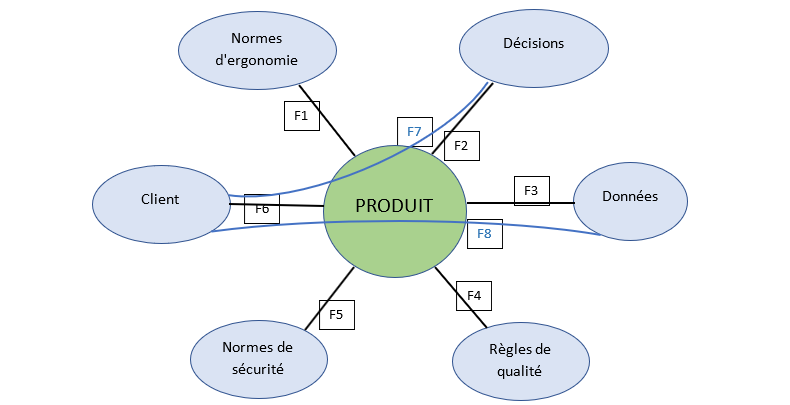
\includegraphics[width=\textwidth]{fsutilisation}
    \caption{Diagramme Pieuvre (Identification des F.S) dans la phase Utilisation}
    \label{fig:fsutilisation}
\end{figure}

On peut formuler 8 fonctions de services d’après le diagramme de la figure \ref{fig:fsutilisation}
\begin{itemize}
    \item Respecter les normes d’ergonomie
    \item Permettre une meilleure prise de décisions
    \item Analyser les données
    \item Respecter les règles de qualité 
    \item Respecter les normes de sécurité
    \item Fournir des indicateurs au client
    \item Permettre au client de prendre les décisions
    \item Permettre au client d'agréger les données
\end{itemize}



\paragraph{Fonctions de service pour la phase de Mise A Jour}

\begin{figure}[H]
    \centering
    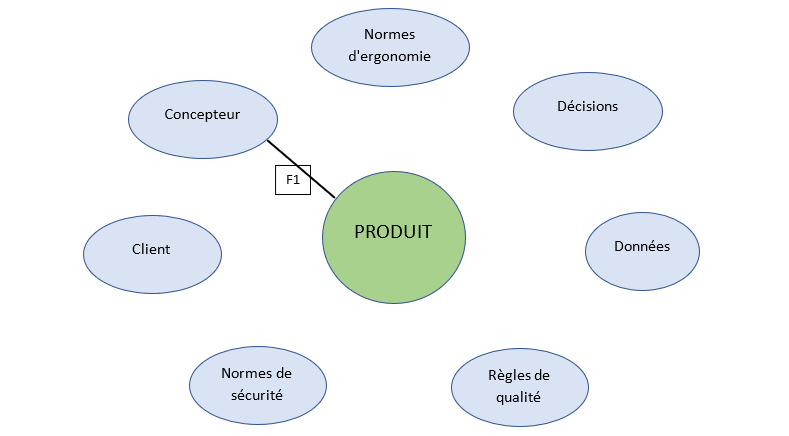
\includegraphics[width=\textwidth]{fsmiseajour}
    \caption{Diagramme Pieuvre (Identification des F.S) dans la phase Mise A Jour}
    \label{fig:fsmiseajour}
\end{figure}



Ici on complémente juste le diagramme precedent. On peut identifier la F.S. suivante dans la figure \ref{fig:fsmiseajour}.
\begin{itemize}
    \item Permettre sa mise à jour par le concepteur
\end{itemize} 



\subsubsection{Le Cahier des Charges Fonctionnel (CdCF)}
Le Cahier des Charges Fonctionnel (CdCF) est le document qui récapitule la démarche et les résultats de l’Analyse Fonctionnelle du Besoin. Il porte donc essentiellement sur les Fonctions de Service. Le CdCF fait office de contrat à respecter par les concepteurs. On doit retrouver dans le CdCF toutes les étapes de la démarche décrite dans ce chapitre :
\begin{itemize}
    \item Identification des phases de vie du produit
    \item Pour chaque phase de vie :
    \begin{itemize}
        \item Identification des EME
        \item Identification des FS 
    \end{itemize}
\end{itemize}

\paragraph{Cahier des Charges Fonctionnel}
\subparagraph{Phases de vie du produit}
\begin{itemize}
    \item Phase d'utilisation
    \item Phase de mise à jour
\end{itemize}
\subparagraph{Eléments du Milieu Extérieur (Cumulé)}
\begin{itemize}
    \item Client (Décideurs) 
    \item Données 
    \item Décisions 
    \item Concepteur
    \item Normes de sécurité 
    \item Normes d'ergonomie
    \item Règles de qualité
\end{itemize}
\subparagraph{Fonctions de Service (Cumulé)}
\begin{itemize}
    \item FS1 - Respecter les normes d’ergonomie
    \item FS2 - Permettre une meilleure prise de décisions
    \item FS3 - Analyser les données
    \item FS4 - Respecter les règles de qualité 
    \item FS5 - Respecter les normes de sécurité
    \item FS6 - Fournir des indicateurs au client
    \item FS7 - Permettre au client de prendre les décisions
    \item FS8 - Permettre au client d'agréger les données
    \item FS9 - Permettre sa mise à jour par le concepteur
\end{itemize}



\subsection{L'Analyse Fonctionnelle Technique (A.F.T.)}

\subsubsection{Définition et intérêt}
L’Analyse Fonctionnelle Technique (A.F.T.) permet de faire la transition entre l’Analyse Fonctionnelle du Besoin (qui reste étrangère aux préoccupations d’ordre technologiques) et la conception détaillée, qui entre de plain pied dans les considérations technologiques. L’Analyse Fonctionnelle Technique est aussi appelée \textbf{Analyse Fonctionnelle interne.}

\paragraph{Intérêts de l’AFT}
\begin{itemize}
    \item \textbf{L’approche systémique : } L’AFT permet une approche systémique de la recherche de solutions technologiques. 
    \item \textbf{La traçabilité : } Les outils de l’AFT permettent aux concepteurs d’associer immédiatement (grâce à son nom) toute Fonction Technique (F.T.) et toute Solution Technologique (S.T.) à la Fonction de Service (F.S.) qui la justifie. Cela permet un suivi optimal du projet/produit durant toute sa vie, y compris pour les évolutions du produit. Si l’on connaît les Fonctions de Service qui sont modifiées, on connaît immédiatement les Solutions Technologiques qui sont impactées par ces modifications.
\end{itemize}



\subsubsection{Le diagramme FAST}
Pour mener une Analyse Fonctionnelle Technique, il existe un outil principal : le F.A.S.T.
(acronyme de « Functionnal Analysis System Technique »). D’autres outils existent, mais il s’agit de
compléments au FAST.

\paragraph{Notion de Fonction Technique :} Une Fonction Technique (F.T.) est une fonction contribuant à réaliser une fonction de service par un moyen technique. Une FT s’énonce nécessairement avec un verbe à l’infinitif. Ce verbe doit être, autant que possible, un verbe d’action.
\begin{itemize}
    \item Toutes les fonctions de service ne peuvent pas être décrites par des FT. Par exemple, une fonction contrainte du type « Respecter la norme », si elle est bien caractérisée, se suffit à elle‐même.
    \item Si l’on n’arrive pas à énoncer une FT avec un verbe d’action, il y a de grandes chances pour que l’on soit en train de faire fausse route.
\end{itemize}

\paragraph{Utilisation du FAST :} Les fonctions, représentées par des blocs rectangulaires, sont liées entre elles par des traits droits (sans flèches), qui les ordonnent. Les fonctions techniques sont nommées \textbf{FT}\textit{ijk}… où i est le numéro de la FS développée (FSi). j et k indiquent la position de la fonction technique dans
l’arborescence de FSi.

Après avoir éliminé les F.S. qui ne respectent pas les règles de formulation de F.T. on peut recenser les F.T. suivants
\begin{itemize}
    \item FS2 - Permettre une meilleure prise de décisions 
    \begin{itemize}
        \item Construire des tableaux de bord
        \item Construire des rapports détaillés
    \end{itemize}
    \item FS3 - Analyser les données
    \begin{itemize}
        \item Construire les cubes de données 
    \end{itemize}
    \item FS8 - Permettre au client d’agréger les données
    \begin{itemize}
        \item Construire un entrepôt de données
    \end{itemize}
\end{itemize}


Image du tableau FAST



\section{Gestion du projet }
\subsection{Processus de développement }
Le processus de développement ou encore cycle de vie, c'est l'ensemble structuré d'activités à réaliser pour atteindre l'objectif d'un projet SI, dont les activités varient en fonction de l'organisation, du projet, et du type de système à développer. Ce processus doit être explicitement décrit pour être adéquatement géré. 
\paragraph{}
Le \textbf{cycle de vie d'un SI} décrit succintement les phases par lesquelles passe un système d'information depuis le \textbf{besoin initial} jusqu'au \textbf{retrait du système}, la documentation et les décisions qui jalonnent le cycle.

\subsubsection{Activités de développement des SI}
\begin{itemize}
    \item \textbf{Spécification} des exigences et des contraintes du système, établissement du cahier des charges
    \item \textbf{Conception} de la solution, production d'un modèle du système à développer
    \item \textbf{Implémentation} du système
    \item \textbf{Test} du système, vérification de l'adéquation entre les propriétés implémentées du système et la spécification des besoins
    \item \textbf{Installation} du système chez le client et vérification de son fonctionnement
    \item \textbf{Maintenance} du système, réparation des fautes
\end{itemize}

\subsubsection{Importance du processus de développement des SI}
Il est important de structurer les phases impliquées dans les efforts de développement de logiciels et le processus de développement sert cet objectif. Le processus de développement ne se termine que lorsque toutes les phases ont été accomplies avec succès. Tous les besoins potentiels doivent être ajustés au sein du système. L'avantage le plus visible du processus de développement est qu'il permet de contrôler dans une certaine mesure les activités de développement et de garantir que le système logiciel est conforme à toutes les exigences estimées. 


\subsubsection{Types de processus de développement}
Il existe plusieurs modèles de cycle de vie (processus de développement) permettant de développer ou de produire des systèmes d’information. Ces modèles ont pour but de détecter les erreurs au pus tôt et ainsi de maitriser la qualité du produit et les délais de réalisation et ainsi que les coûts de réalisation. On peut regrouper ces modèles de cycle de vie en trois catégories soit :
\begin{itemize}
    \item \textbf{Les modèles linéaires :}  Il se compose d'un certain nombre de phases qui sont exécutées dans un ordre séquentiel sans boucles de rétroaction. Il ne produit une solution qu'à la fin phase.
    \item \textbf{Les modèles itératifs :} Il se compose d'un certain nombre de phases qui sont répétés en groupes avec un feedback après l'exécution de chaque groupe.
    \item \textbf{Les modèles agiles :} Modèle adaptatif, progresse d'itération en itération basé sur une spécification limitée de la solution. Chaque itération apprend des précédentes et redirige l'tération suivante pour tenter de converger vers la meilleure solution possible capabl de satisfaire le client.
\end{itemize}

Aujourd’hui, la catégorie des méthodes agile est plus répandue par rapport aux deux autres car elle permet l’aboutissement d’un produit qui satisfait mieux le client, plus facilement modifiable et beaucoup moins couteux pour la maintenance et la mise a jour que les autres.\\
Dans cette catégorie nous pouvons recenser quelques-uns des méthodes les plus utilisées :


\begin{itemize}
    \item \textbf{Méthodologie Agile Scrum : } Scrum  est un cadre de gestion de projet Agile léger qui peut être utilisé pour gérer des projets itératifs et incrémentiels de tous types. Il a gagné en popularité au fil des ans en raison de sa simplicité, de sa productivité éprouvée et de sa capacité à intégrer diverses pratiques globales promues par d'autres modèles Agile.
    \item \textbf{Kanban : } Kanban  est une méthode de gestion de flux de travail hautement visuelle qui est populaire parmi les équipes Lean. En effet, 83\% des équipes pratiquant le Lean utilisent Kanban pour visualiser et gérer activement la création de produits en mettant l'accent sur la livraison continue, sans ajouter plus de stress au cycle de vie du développement logiciel.
    \item \textbf{Extreme Programming (XP) : } XP est une approche disciplinée pour le développement de logiciels agiles de haute qualité, axée sur la rapidité et la livraison continue. Il vise à améliorer la qualité et la réactivité des logiciels face à l'évolution des exigences des clients. Il favorise une forte implication des clients, de feedback rapide, des tests continus, une planification continue et un travail d'équipe étroit pour fournir des logiciels fonctionnels à des intervalles très fréquents, généralement toutes les 1 à 3 semaines.
\end{itemize}

Pour ce projet nous utiliseront la méthodologie SCRUM car elle est la plus adaptée pour la gestion de notre projet.

% \subsection{Choix des outils de modélisation}
% \blindtext


\subsection{Outils et techniques de gestion}
\subsubsection{Présentation du processus de développement agile : SCRUM}
\paragraph{Principes de SCRUM}
Scrum est considéré comme un cadre ou « framework » de gestion de projet. Ce cadre est constitué d'une définition des rôles, de réunions et d'artefacts.

Scrum définit 3 rôles :​
\begin{itemize}
    \item \textbf{Le « Product Owner »} qui porte la vision du produit à réaliser (représentant généralement le client).
    \item \textbf{Le « Scrum Master »} garant de l'application de la méthodologie Scrum.
    \item \textbf{L'équipe de développement} qui réalise le produit.
\end{itemize}

\paragraph{Cycle de vie SCRUM}
\subparagraph{Un peu de vocabulaire :}
\begin{itemize}
    \item \textbf{Product backlog (Backlog produit) : } Une liste priorisée de besoins et exigences que veut le client, exprimé dans son vocabulaire et sa terminologie métier, souvent en termes de scénarios (user stories).
    \item \textbf{User story (scénario) : }Le scénario est une exigence du système à développer, formulée en une ou deux phrases dans le langage de l'utilisateur. Ces user stories émergent au cours d'ateliers de travail menés avec le Métier, le Client et/ou les utilisateurs.
    \item \textbf{Sprint backlog : }Une liste de tâches identifiées par l'équipe du projet à réaliser pendant un sprint afin d'implémenter les scénarios sélectionnés pour ce sprint.
    \item \textbf{Daily scrum : }Chaque jour on organise une courte réunion (15 minutes) pour fixer et/ou ajuster les objectifs de la journée.
\end{itemize}

La vie d'un projet Scrum est rythmée par un ensemble de réunions clairement définies et strictement limitées dans le temps (timeboxing):
\begin{itemize}
    \item \textbf{Planification du Sprint (Sprint = itération) :} Au cours de cette réunion, l'équipe de développement sélectionne les éléments prioritaires du \textbf{« Product Backlog »} (liste ordonnancée des exigences fonctionnelles et non fonctionnelles du projet) qu'elle pense pouvoir réaliser au cours du sprint (en accord avec le \textbf{« Product Owner »}).
    \item \textbf{Revue de Sprint : } Au cours de cette réunion qui a lieu à la fin du sprint, \textbf{l'équipe de développement} présente les fonctionnalités terminées au cours du sprint et recueille les feedbacks du \textbf{Product Owner} et des utilisateurs finaux. C'est également le moment d'anticiper le périmètre des prochains sprints et d'ajuster au besoin la planification de release (nombre de sprints restants).
    \item \textbf{Rétrospective de Sprint : }La rétrospective qui a généralement lieu après la revue de sprint est l'occasion de s'améliorer (productivité, qualité, efficacité, conditions de travail, etc) à la lueur du "vécu" sur le sprint écoulé (principe d'\textbf{amélioration continue}).
    \item \textbf{Mêlée quotidienne : }il s'agit d'une réunion de synchronisation de l'équipe de développement qui se fait debout (elle est aussi appelée "stand up meeting") en 15 minutes maximum au cours de laquelle chacun répond principalement à 3 questions : « Qu'est ce que j'ai terminé depuis la dernière mêlée ? Qu'est ce que j'aurai terminé d'ici la prochaine mêlée ? Quels obstacles me retardent ? »
\end{itemize}
\begin{figure}[H]
    \centering
    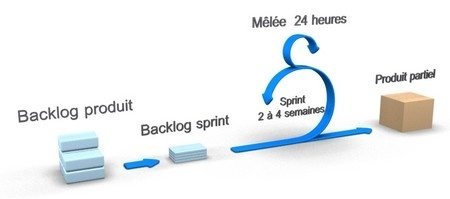
\includegraphics[width=\textwidth]{scrum}
    \caption{Cycle de vie de SCRUM}
    \label{fig:scrum}
\end{figure}

Comme on le vois dans la figure \ref{fig:scrum}, durant chaque "sprint" (habituellement 2-4 semaines), l'équipe crée un livrable. L'ensemble des fonctionnalités du sprint viennent du "backlog" du projet, qui est un ensemble priorisé d'exigences importantes à achever. Pendant une session de planification de sprint, les exigences du sprint sont définies. Les exigences sont gelées pendant un sprint. Le sprint doit finir à temps. Si les exigences ne sont pas totalement mises en place, elles retournent au backlog du projet. Après avoir complété un sprint, l'équipe doit démontrer le fonctionnement du logiciel.

\subparagraph{Avantages : }
\begin{itemize}
    \item Économie de temps et d'argent ;
    \item Mise en place rapide et facilité de correction des possible erreurs ;
    \item Visibilité de la mise en place du projet ;
    \item Feedback en continu du client ;
    \item Facilité de copie avec les changements ;
    \item Les réunions journalières amènent à meilleure appréciation de la productivité individuelle ;
    \item Les problèmes sont identifiés dans les premières étapes, de manière à être résolus plus rapidement ;
    \item Il est plus facile de livrer un produit de qualité durant un temps planifié.
\end{itemize}

\subsubsection{Technique d’estimation des coûts}
Afin d’évaluer le coût de notre projet, on doit d’abord définir les éléments de base qui constitue votre projet : 
\begin{itemize}
    \item Le planning initial du projet
    \item La durée de chaque tâche
    \item La durée totale du projet
    \item Les ressources humaines nécessaire
    \item Les ressources matérielles nécessaire
    \item Les ressources logiciels nécessaire
\end{itemize}

\paragraph{Méthodes d’estimation des coûts : }On distingue deux méthodes
\begin{itemize}
    \item \textbf{La méthode analogique :} Cette méthode consiste à se référer aux coûts réels des projets similaires au vôtre et à les adapter en faisant quelques ajustements. Il est également possible de s’appuyer sur l’avis d’un chef de projet expérimenté qui a travaillé sur un projet semblable. Elle se déroule en trois étapes :
    \begin{itemize}
        \item Analyse du projet ;
        \item Recherche d’un projet similaire ;
        \item Comparaison et chiffrage.
    \end{itemize}
    \item \textbf{La méthode ascendante :} Le but de cette méthode est d’estimer le coût de chaque groupement de tâches, puis d’additionner chacune de ces estimations afin d’obtenir le coût global du projet. Cette méthode est plus précise que la précédente car elle s’appuie sur l’expérience et l’avis des personnes qui exécutent les tâches en question. Cette méthode s’utilise lors de l’élaboration du budget. Une fois que tous les éléments du projet ont été chiffrés, on les additionne afin d’obtenir le coût total du projet.
\end{itemize}

Nous optons pour la deuxième méthode pour plus de précision.

\subsubsection{Outils collaboratifs}
Des centaines d’outils collaboratifs existent pour toute sorte de collaboration. Nous allons nous attarder sur trois catégories nous permettant de mener à bien notre projet. 

\paragraph{Outil de gestion de projet : }Ici nous avons opte pour \textbf{Trello}. Cet espace collaboratif prend la forme de « boards » pour les projets ou clients et de « cards » pour les tâches. Trello vous permet ainsi de suivre l’avancée des différentes missions des prestataires. Vous pouvez, par exemple, avoir une colonne « À faire », « En cours », « Rendu » et « Validé ». Lorsque vous serez en train de travailler sur une tâche, il pourra la glisser dans « En cours », puis dans « Rendu » lorsque c’est terminé. De cette façon on peut tracer et savoir exactement l’état d’avancement du projet ainsi que des taches qui bloquant l’avancement ou même des idées susceptibles d’améliorer le projet.

\paragraph{Outil professionnel pour la communication dans l’équipe : } Nous avons choisi \textbf{Slack} ici. Slack est une application de messagerie instantanée permettant le travail collaboratif. Les conversations avec vos collaborateurs et prestataires sont organisées sous forme de chaînes et lorsque l’écrit ne suffit plus vous pouvez facilement organiser des appels audios et/ou vidéos.
 \paragraph{Outil professionnel pour les réunions : } \textbf{Skype} est un logiciel de messagerie instantanée utile pour dialoguer avec vos collaborateurs en temps réel. Vous pourrez facilement organiser des réunions, et même partager vos écrans et annoter des présentations PowerPoint. Les fonctionnalités de Skype sont très avancées pour le travail collaboratif.
\subsection{Planning prévisionnel}
\subsubsection{Planification du projet}
\blindtext

\subsection{Estimation des coûts}
\blindtext

\subsubsection{Couts de développement}
\blindtext

\subsubsection{Cout de mise en production}
\blindtext



\section*{Conclusion}%
\addcontentsline{toc}{section}{\numberline{}Conclusion}%
\blindtext
